%!TEX root=../main.tex
\section{Application} % (fold)
\label{sec:application}

\textcolor{red}{We implement our methodology utilizing data from the National Basketball Association (NBA). To access comprehensive game data, we utilize the Python package \texttt{nba\_api}\footnote{\url{https://github.com/swar/nba_api/}}, which provides access to the APIs of \url{nba.com}. The dataset encompasses shot location data from all NBA games spanning the seasons between $2018-2019$ and $2022-2023$. Filtering the dataset, we focus solely on players who have made more than $1000$ shots during this five-season period, resulting in a cohort of $131$ players. These players accounted for a total of $493723$ shots attempted, of which $234941$ were successful. Subsequently, we exclude shots deemed impossible (e.g., out-of-bounds), leaving us with a dataset comprising $492621$ shots. To analyze shooting behavior, we employ 2-dimensional kernel density estimation, utilizing Silverman's rule \citep{silvermanDensityEstimationStatistics1986} for bandwidth estimation. The density estimation is conducted on a regularly spaced grid consisting of $51 \times 51$ points.}

\begin{figure}
    \centering
    \begin{subfigure}[b]{0.49\textwidth}
        \centering
        \includegraphics[width=\textwidth]{figures/curry_make_miss.pdf}
        \caption{Stephen Curry}
        \label{fig:curry_make_miss}
    \end{subfigure}
    \hfill
    \begin{subfigure}[b]{0.49\textwidth}
        \centering
        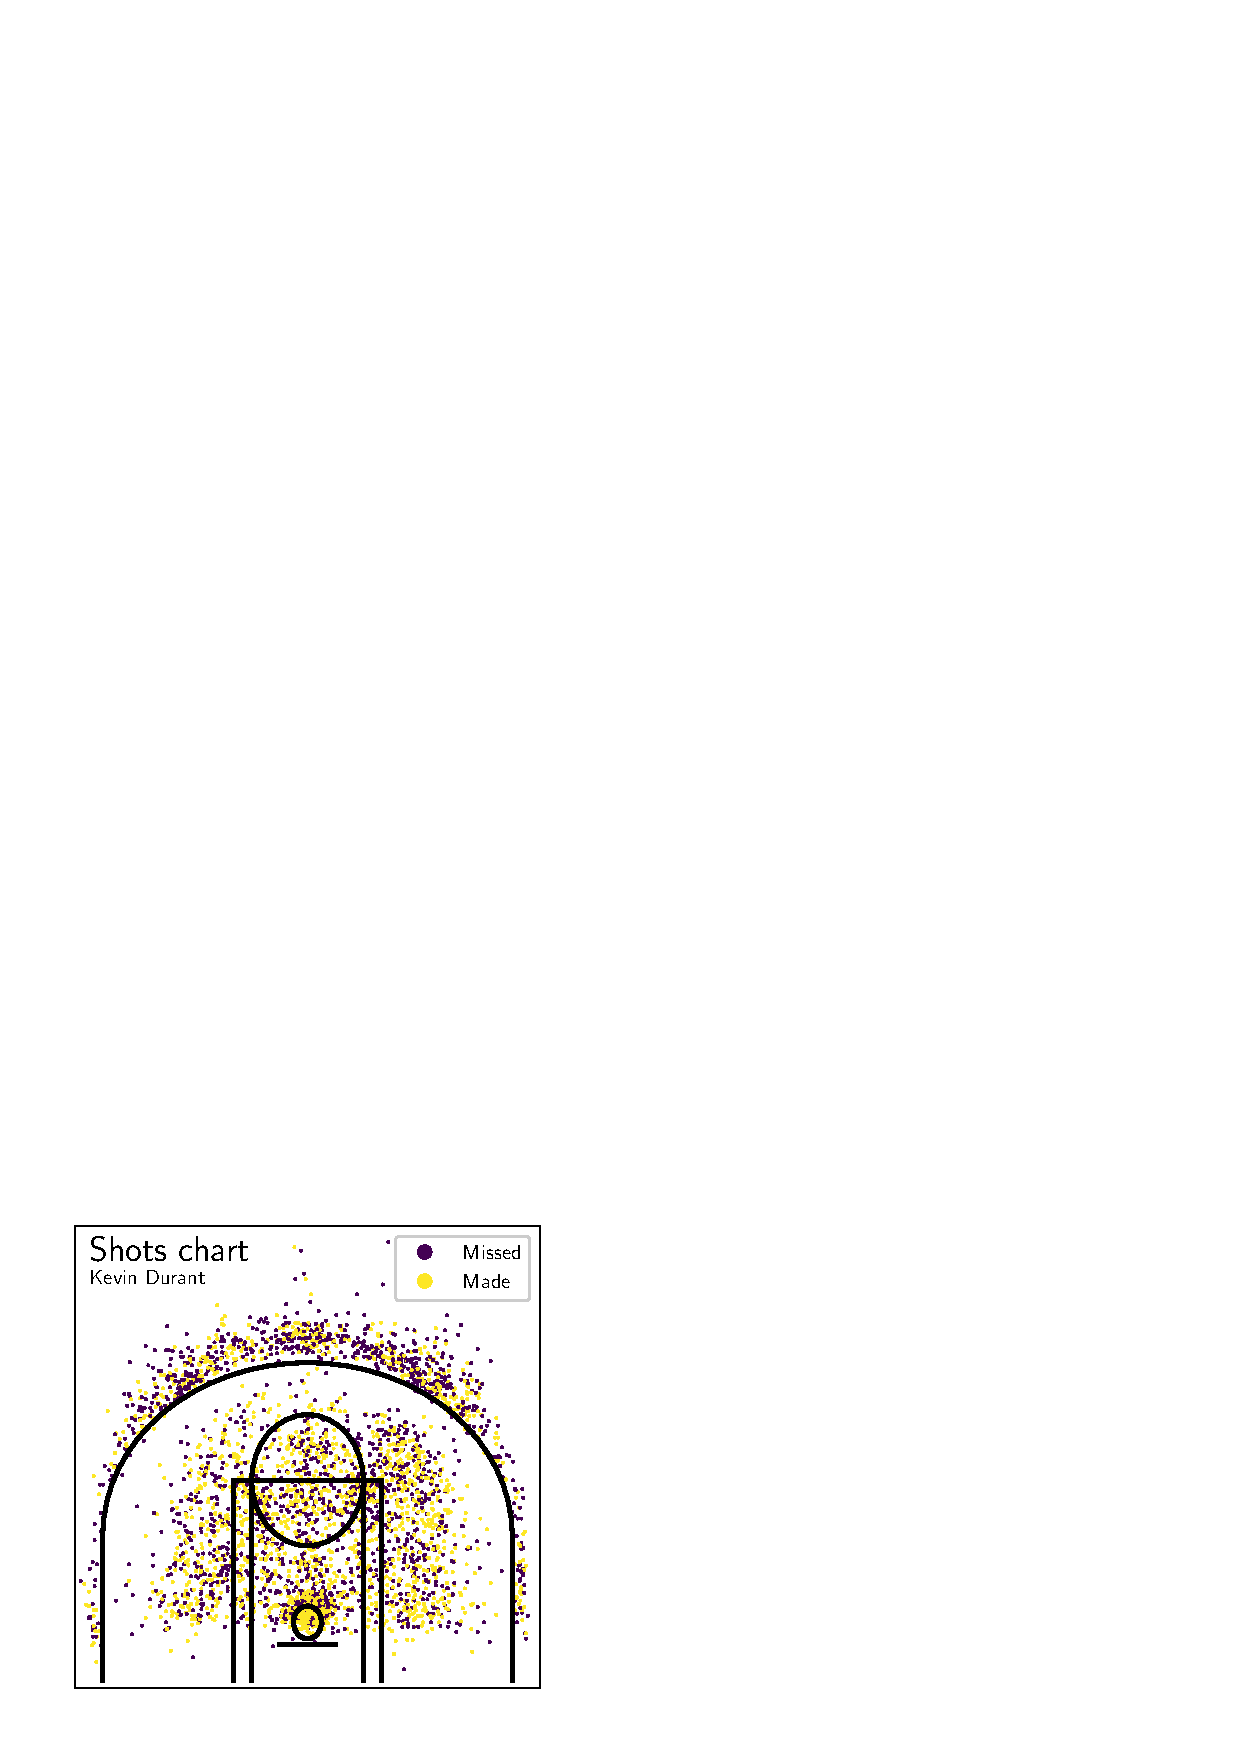
\includegraphics[width=\textwidth]{figures/durant_make_miss.pdf}
        \caption{Kevin Durant}
        \label{fig:durant_make_miss}
    \end{subfigure}
    \caption{Make/Miss chart for Stephen Curry and Kevin Durant.}
    \label{fig:shoots_make_miss}
\end{figure}


\textcolor{red}{We estimate the principal components using the decomposition of the Gram matrix and the eigenanalysis of the covariance operator using the FCP-TPA for the univariate components. Figure \ref{fig:curry_shoots_decomposition} shows examples of the shooting densities of Stephen Curry and their first five functional principal components using both methods (Figure \ref{fig:curry_decomposition} for the Gram matrix decomposition and Figure \ref{fig:curry_decomposition_fcptpa} for the MFPCA with FCP-TPA. Remark that the functional principal components, as a representation of the deviation from the mean surface function, may take negative values, while density can only take positive values. For presentation purpose, the functional principal components have been normalized between $-1$ and $1$. Blue corresponds to negative values of the functional components, and thus contribute negatively to the density, whil Red corresponds to positive values of the functional components, and thus contribute positively to the density. The bluer the area in the image of the functional components, the smaller/negative the scores, whereas the redder areas correspond to positive values of the scores. The white areas correspond to scores that are closed to $0$, and basically have not impact on the density. The obtained functional components can be explained as different shooting styles.}
\begin{figure}
    \centering
    \begin{subfigure}[b]{0.45\textwidth}
        \centering
        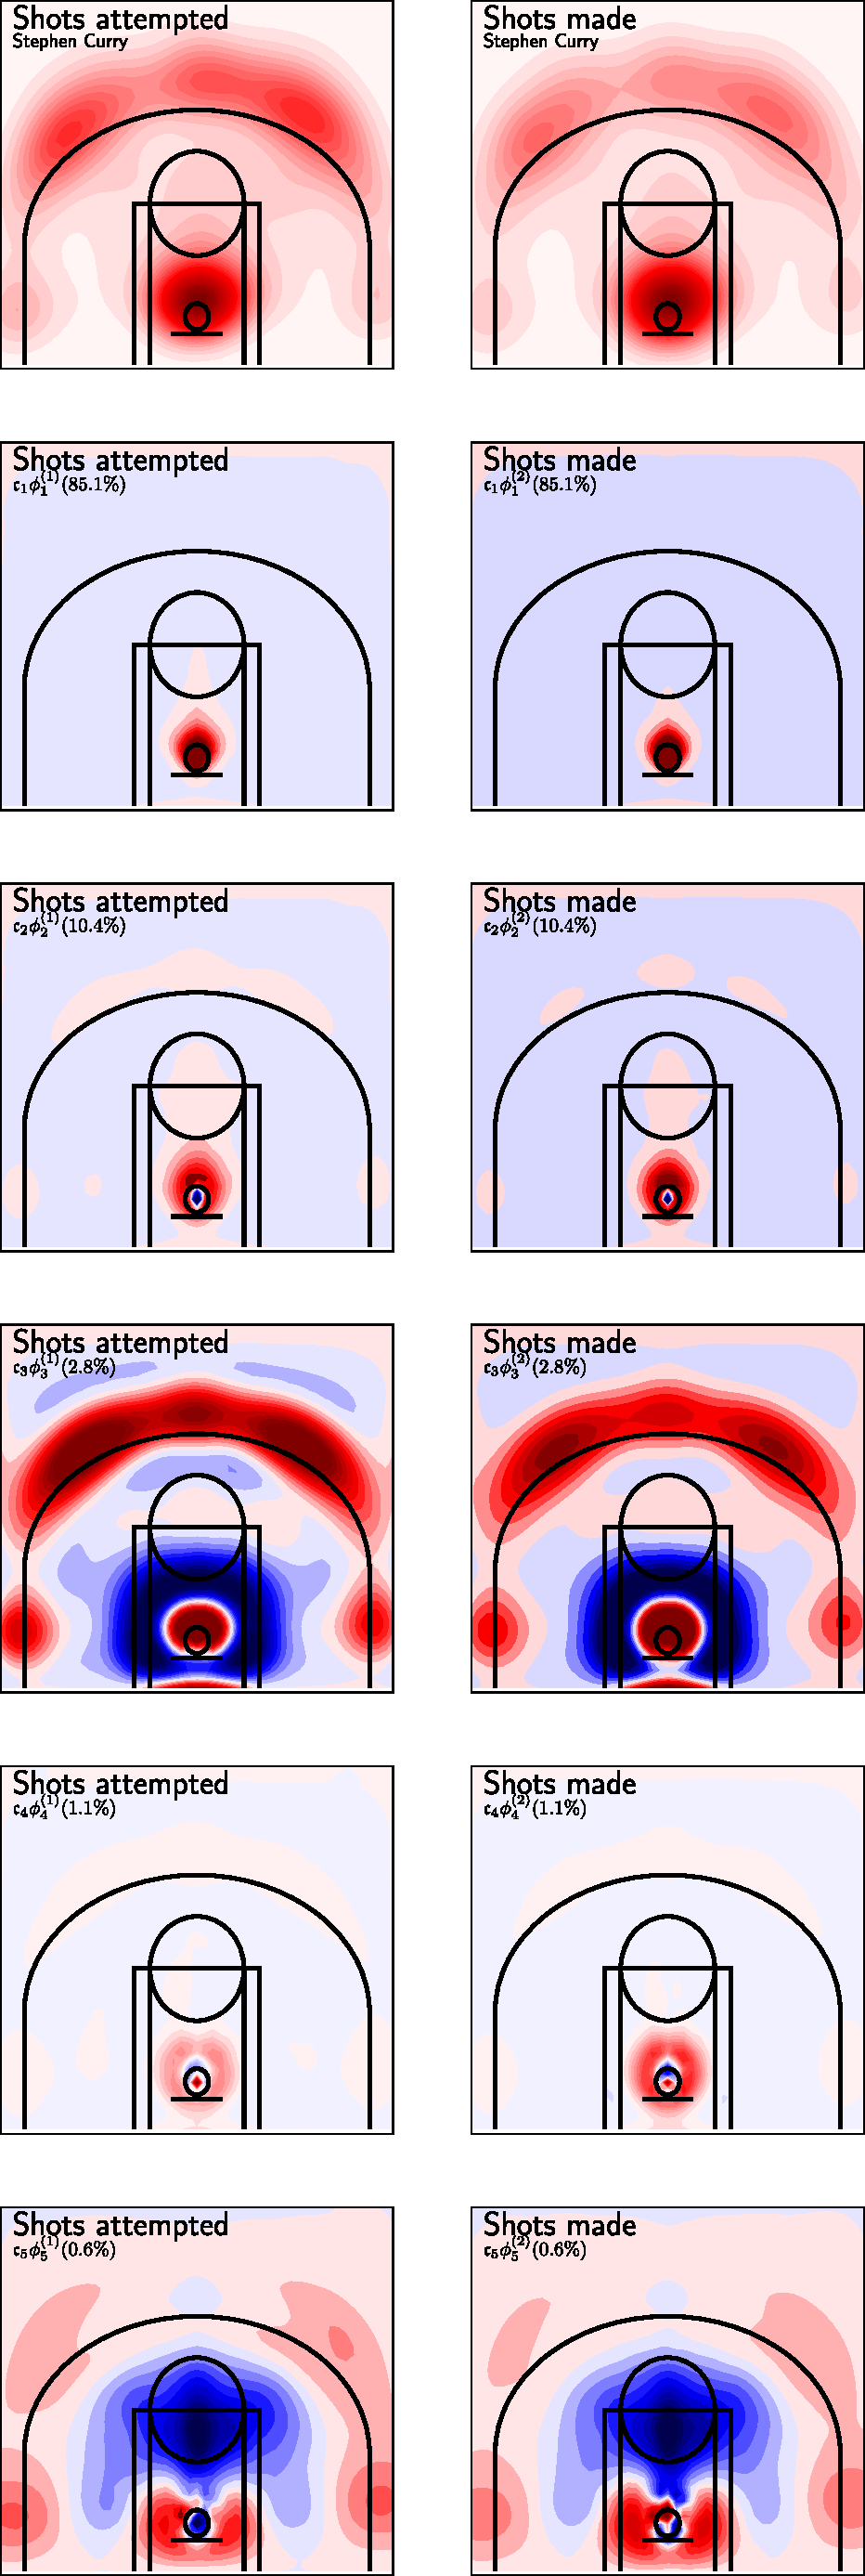
\includegraphics[width=\textwidth]{figures/curry_decomposition.pdf}
        \caption{Gram matrix}
        \label{fig:curry_decomposition}
    \end{subfigure}
    \hfill
    \begin{subfigure}[b]{0.45\textwidth}
        \centering
        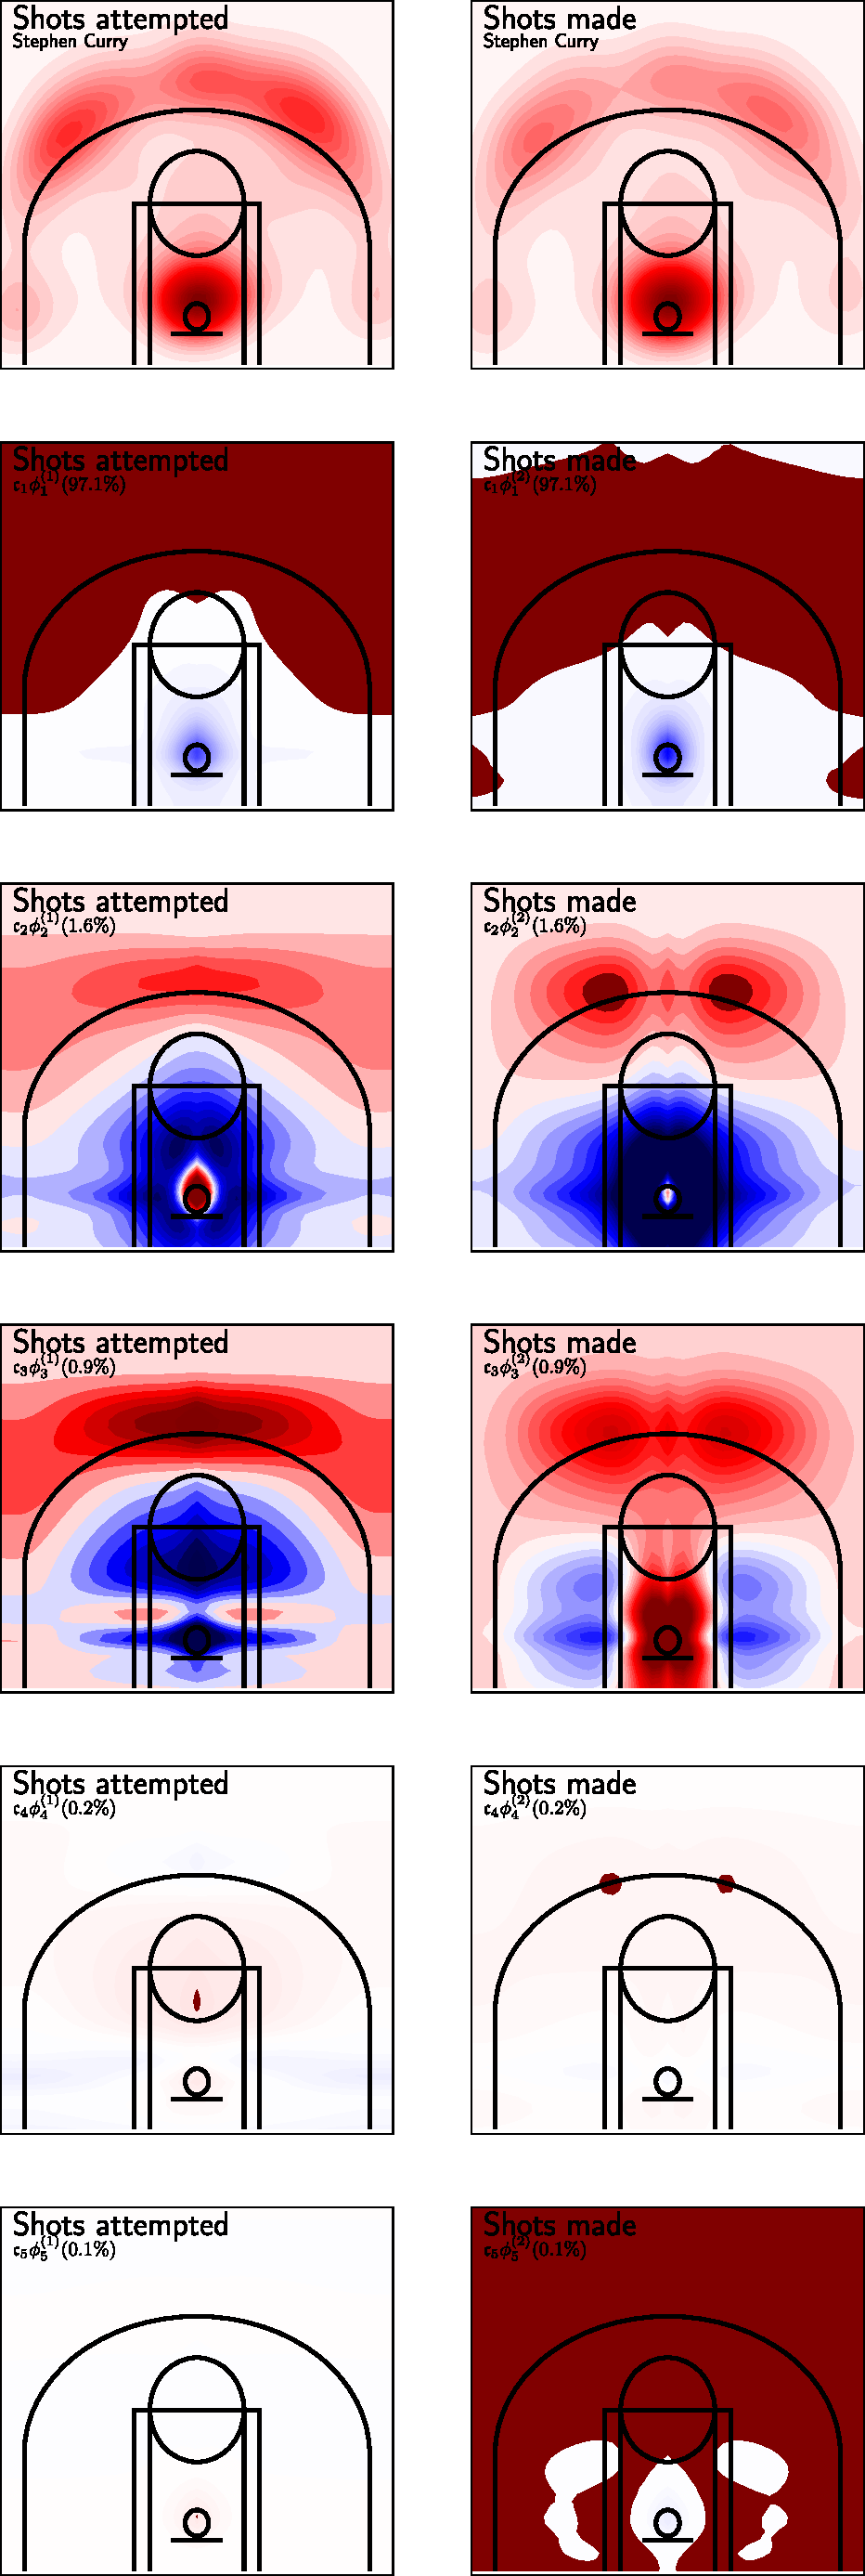
\includegraphics[width=\textwidth]{figures/curry_decomposition_fcptpa.pdf}
        \caption{FCPTPA}
        \label{fig:curry_decomposition_fcptpa}
    \end{subfigure}
    \caption{Decomposition for Stephen Curry.}
    \label{fig:curry_shoots_decomposition}
\end{figure}
\textcolor{red}{For the Gram matrix, the first two principal components and the fourth are related to the shoots under the basket, excluding the other areas. This account for around $95\%$ of the variance. The third and fifth components are related to the three-pointers. These results exhibits the shooting patterns of Stephen Curry. He mostly scores under the basket or behind the three-points line, but almost never in-between. The decomposition of the density of made shots is similar to the ones of attempted shots. We may advance an explanation for that: Stephen Curry does not have a ``weak'' spot, that is somewhere on the court where he shots a lot but does not score.}
% section application (end)